\begin{figure}[ht]
\centering
\vspace{-6mm}
\centerline{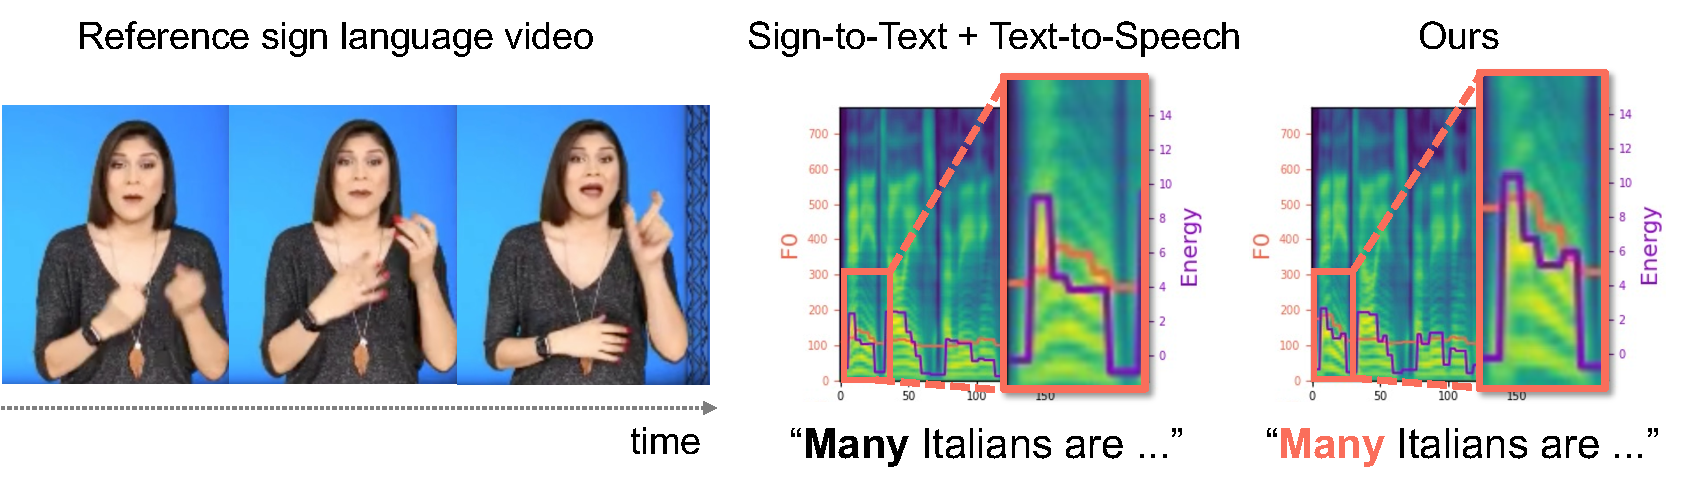
\includegraphics[width=\linewidth]{assets/heading.pdf}}
\vspace{-5mm}
\caption{
% We propose S2PFormer for \emph{Sign-to-Speech Prosody Transfer} task. 
% Our key idea is to directly transfer the sign language prosody into speech synthesis by ensuring that the prosodic cues of the sign language can be reconstructed from the synthesized speech.
In the reference sign language video (left), the first phrase, ``many Italians,'' is emphasized through rapid hand movements and facial expressions. The two-stage baseline (middle) fails to reflect this prosody, whereas our approach (right) successfully captures the emphasis on ``many.''}
\vspace{-8mm}
\label{fig:pipeline}
\end{figure}